\documentclass[tikz, border = 10pt]{standalone}
\renewcommand{\familydefault}{\sfdefault} 

\usetikzlibrary{positioning, quotes, calc, arrows.meta, bending, shapes, backgrounds}

\tikzset{
every node/.style = {scale = 1.1},
manifest/.style = {rectangle, draw, thin, inner sep = 5pt, minimum width = 1cm, 
	minimum height = 1cm},
latent/.style = {ellipse, draw, thin, inner sep = 5pt, minimum width = 1cm, 
	minimum height = 1cm},
residual1/.style = {circle, draw, thin, minimum size = 5mm, inner sep = 1pt}, 
residual2/.style = {rectangle, minimum width = 0.5pt, minimum height = 1.5mm, 
	inner sep = 0pt, outer sep = 0mm},
regression/.style = {-{Stealth[length = 1.5mm]}, thin, shorten > = 1pt, inner sep = 2pt},
covariance/.style={{Stealth[length = 1.5mm]}-{Stealth[length = 1.5mm]}, thin, 
	shorten > = 1pt, shorten < = 1pt, inner sep = 2pt},
variance/.style={{Stealth[length = 1mm]}-{Stealth[length = 1mm]}, thin, 
	shorten > = 1pt, shorten < = 1pt, inner sep = 1.5pt},
interaction/.style = {-{Stealth[sep = 1pt, length = 1.5mm] . Circle[length = 4pt]}, 
	thin, shorten > = -2pt},
constant/.style = {draw, thin, inner sep = 1pt, regular polygon, 
    regular polygon sides = 3, minimum size = 5mm}
}
\usetikzlibrary{positioning, quotes, calc, arrows.meta, bending, shapes, backgrounds}
\renewcommand{\familydefault}{\sfdefault} 
\definecolor{orange}{HTML}{CB6015}

\begin{document}
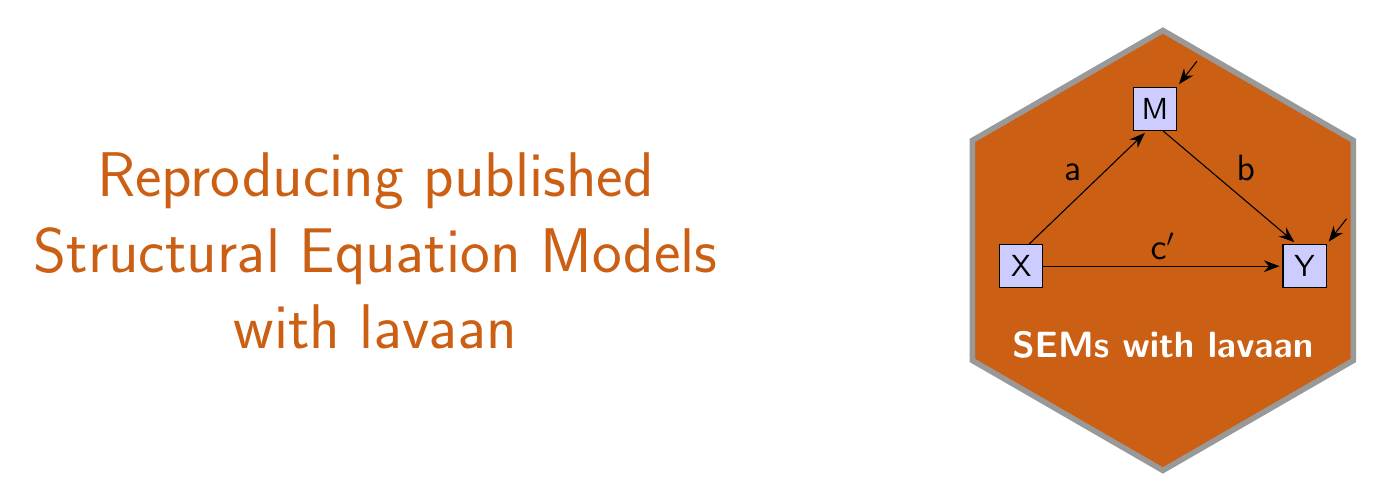
\begin{tikzpicture}

\tikzset{
manifest/.style = {rectangle, draw,  inner sep = 2pt, minimum width = 0.5cm, 
	minimum height = 0.5cm, fill = blue!20},
residual/.style = {rectangle, minimum width = 0.5pt, minimum height = 1.5mm, 
	inner sep = 0pt, outer sep = 0mm},
regression/.style = {-{Stealth[length = 2mm]}, shorten > = 1pt, inner sep = 2pt},
	}

%% Hexagon
\node (hexagon) [draw, color = black!40, fill = orange, line width = 2pt, regular polygon, regular polygon sides = 6, rotate = 30, minimum size=5.08cm, ] {};

%% SEM
% Manifest
\node at (-1.8, -0.2) [manifest] (X) {X};
\node at (1.8, -0.2) [manifest] (Y) {Y};
\node at (-.1, 1.8) [manifest] (M) {M};

% The regressions
\path [regression] (X) edge ["\large{c$'$}"] (Y);
\path [regression] (X.70) edge ["\large{a}"] (M.250);
\path [regression] (M.290) edge ["\large{b}"] (Y.110);

% The residuals
\node [residual] (e2) [above right = 2.5mm and 2.5mm of Y] {};
\node [residual] (e1) [above right = 2.5mm and 2.5mm of M] {};
\path [regression] (e2) edge (Y.north east);
\path [regression] (e1) edge (M.north east);

%% Label
\draw (0, -1.2) node [text = white] {\bf\large{SEMs with lavaan}};

%% Heading
\node at (-10, 0) [inner sep = 2pt, font = \huge, align = center, color = orange] (header) 
     {Reproducing published\\Structural Equation Models\\with lavaan};

\end{tikzpicture}
\end{document}